\chapter{PGF and TikZ}

PGF ("Portable Graphics Format") and TikZ ("TikZ ist kein Zeichenprogramm") are powerful tools used to create high-quality diagrams directly within LaTeX.

TikZ is the user-facing layer that provides an intuitive syntax to create graphics. PGF is the lower-level layer responsible for the rendering. Most users interact primarily with TikZ, which internally compiles down to PGF commands. In short:

\begin{itemize}
    \item \texttt{TikZ} is easier to write and read.
    \item \texttt{PGF} handles the rendering and offers more fine-grained control (often used via libraries like \texttt{pgfplots}).
\end{itemize}

\section{Baby's first \texttt{tikzpicture}}

This example draws a simple equilateral triangle using absolute coordinates. It shows how to connect points with lines and place text within the diagram. This kind of drawing is useful for basic geometric figures or quick sketches.

\begin{center}
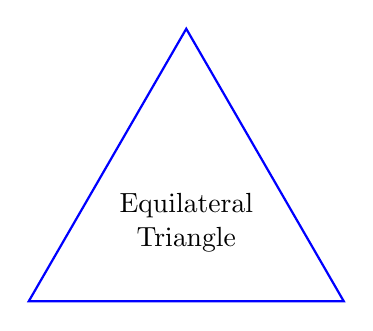
\begin{tikzpicture}
    \draw[thick, blue] (0,0) -- (4,0) -- (2,3.46) -- cycle;
    \node[align=center] at (2,1) {Equilateral \\ Triangle};
\end{tikzpicture}
\end{center}

\section{Flowchart with TikZ}

Here we use named nodes and relative positioning to create a simple flowchart. This style makes it easier to maintain and adjust diagrams without dealing with raw coordinates. Shapes like diamonds (used here for decisions) are part of TikZ's geometric shapes library.

\begin{center}
\begin{tikzpicture}[node distance=1.5cm and 2cm, every node/.style={draw, align=center, minimum width=2cm}]
    \node (start) {Start};
    \node[below=of start] (process) {Process};
    \node[below=of process] (decision) [diamond, aspect=2] {Decision?};
    \node[below left=of decision] (yes) {Yes};
    \node[below right=of decision] (no) {No};

    \draw[->] (start) -- (process);
    \draw[->] (process) -- (decision);
    \draw[->] (decision) -- (yes);
    \draw[->] (decision) -- (no);
\end{tikzpicture}
\end{center}

\section{Diagrams with PGFPlots}

This example uses the \texttt{pgfplots} package (built on top of PGF) to plot a mathematical function. PGFPlots is ideal for data visualization and produces publication-quality plots. This one handles scaling, grid lines, and sampling automatically.

\begin{center}
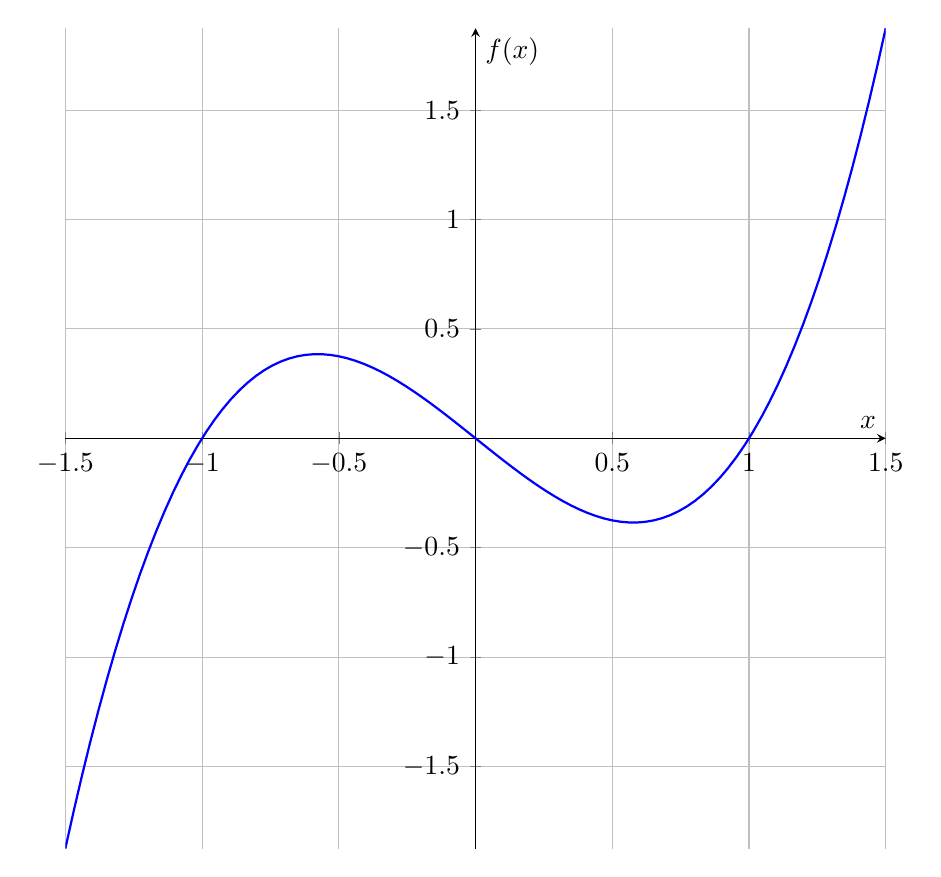
\begin{tikzpicture}
    \begin{axis}[
        axis lines=middle,
        height=12cm,
        width=12cm,
        xlabel={$x$},
        ylabel={$f(x)$},
        grid=both,
        domain=-1.5:1.5,
        samples=100,
        ]
        \addplot[blue, thick] {x^3 - x};
    \end{axis}
\end{tikzpicture}
\end{center}

\clearpage
\section{Plotting External Data}

PGFPlots also allows importing data from external files such as CSVs, which is common in scientific documents. Below is a plot of temperature readings taken during a 1-hour experiment at 5-minute intervals.

Make sure the CSV file is accessible and contains headers matching those referenced in the plot code.


\begin{center}
\begin{tikzpicture}
    \begin{axis}[
        xlabel={Time (min)},
        ylabel={Temperature (°C)},
        thick,
        ]
        \addplot[blue] table [
            col sep=comma,
            x={Time (min)},
            y={Temperature (°C)}
            ] {data/temperature_measurement.csv};
    \end{axis}
\end{tikzpicture}


\begin{tikzpicture}
    \begin{axis}[
        xlabel={Time (min)},
        ylabel={Temperature (°C)},
        ymax=45,
        xmin=0,
        ymin=0,
        grid=both,
        ]
        \addplot[blue] table [
        col sep=comma,
        x={Time (min)},
        y={Temperature (°C)}
        ] {data/temperature_measurement.csv};
    \end{axis}
\end{tikzpicture}
\end{center}

\clearpage
\section{Distinct Line Styles}

In academic or black-and-white printing, it is often necessary to distinguish plot lines using different styles (e.g., dashed, dotted) instead of color. This is particularly useful for accessibility or publication constraints. Below is an example showing \texttt{sin(x)} and \texttt{cos(x)} using distinct dash patterns.

\begin{center}
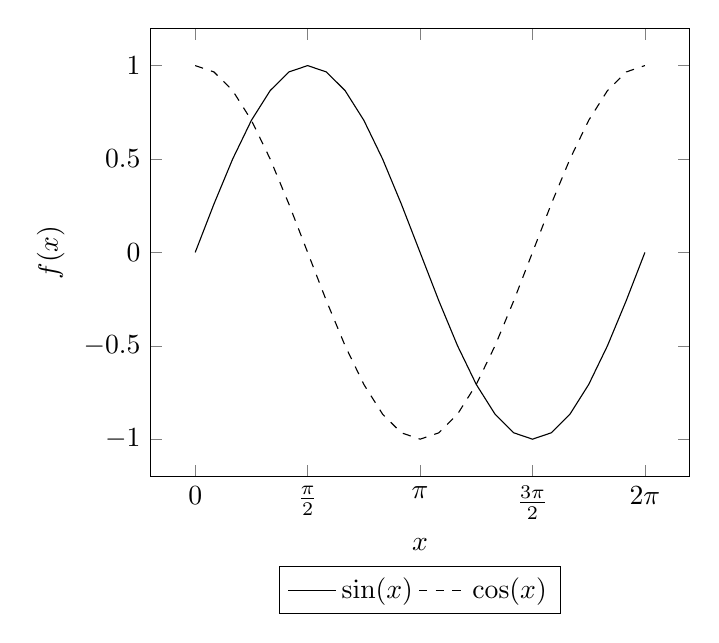
\begin{tikzpicture}
    \begin{axis}[
        xlabel={$x$},
        ylabel={$f(x)$},
        xtick={0, 1.571, 3.142, 4.712, 6.283},
        xticklabels={$0$, $\frac{\pi}{2}$, $\pi$, $\frac{3\pi}{2}$, $2\pi$},
        ytick distance=0.5,
        domain=0:6.283,
        legend style={at={(0.5,-0.2)}, anchor=north, legend columns=-1},
        ]
            \addplot[solid] {sin(deg(x))};
            \addlegendentry{$\sin(x)$}

            \addplot[dashed] {cos(deg(x))};
            \addlegendentry{$\cos(x)$}
    \end{axis}
\end{tikzpicture}
\end{center}
